% \section{Model Driven Engineering}

Model Driven Engineering (MDE) has emerged as a central paradigm in software development. 
It's history is intertwined with that of Object Oriented Programming (OOP). 
Where the OOP paradigm can be summarized as \textit{everything is an object}, MDE is similarly described as the paradigm where \textit{everything is a model}. 
Two of the longest standing actors are the Object Management Group (OMG) which notably provides specifications for both the Unified Modeling Language and the Object Constraint Language, and Eclipse providing the Eclipse Modeling Framework (EMF).
EMF allows for the generation and testing of code using UML specifications, the design and use domain specific languages, and the manipulation of data by means of model transformation.
More recent efforts include JetBrains' Meta Programming System (MPS) which focuses on providing tools to develop and use Domain Specific Languages.

Models are used because they are: cheaper, safer, easier to manipulate and learn from.
For software development, software engineers build models of the desired software.
Such models allow the engineers to quickly iterate and test their design, 
but also serve as a language to communicate with the software developers who will implement the software. 
Beyond software development, models are similarly used: 
scaled-down models of buildings are easier to make and iterate upon and can be used to communicate with stake holders,
weather models provide forecasts which are crucial to farming,
digital-twins allow for the monitoring and interaction with complex systems.

% All of these efforts rely on the same theoretical foundations, which is outlined in the first section.
In the following sections we'll present UML and OCL.
We'll then present the state-of-the-art for MDE, and the tools we are building upon.

% \section{Fundamentals of Formal Modeling}
% In this section we present formal foundations the MDE framework required for the problem of model search.
The concepts in this section are primerily distilled from the Object Managament Group's Meta-Object Facility.

%%%%%%%%%%%%
% Model
%%%%%%%%%%%%
\subsection{Object Models}
At the center of Model Driven Engineering is the concept of \textit{model}.
Models represent \textit{systems under study}.
This relation between model and system under study, is named \textit{represents} and is given the symbol $\mu$.

\begin{figure}[h]
    \centering
    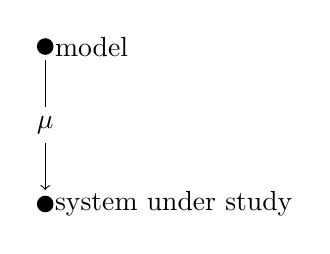
\begin{tikzpicture}
        \coordinate [label=0:{system under study}] (M) at (0,0);
        \coordinate [label=0:{model}]  (MM) at (0,2);
      
          \fill (M) circle (3pt);
          \fill (MM) circle (3pt);
          
        \draw[->, shorten <= 5pt, shorten >= 5pt,] (MM) -- (M) node [midway,fill=white] {$\mu$};
    \end{tikzpicture}
    \caption{$\mu$: \textit{a model represents a system under study}}
\end{figure}

Models often represent only part of the system under study, especially when the system under study is very complex.

\subsubsection{Definitions}

\noindent
\textbf{Object}: 
an object is an entity that identifies information.
Objects can represent things from the real world, or abstract concepts.
Objects are uniquely identifiable.
Objects can be associated, composed or otherwise linked.
For instance, an object can be used to represent a person: with properties such as their name or age, or their links to other people.

\noindent
\textbf{Object Property}: a named collection of elements, representing information from the system under study.
Depending on the type of elements, a property is either an attribute or a reference.

\noindent
\textbf{Property Access}: the process of access the information indentified by an object.
These kind of functions are often called \textit{getters} and \textit{setters}:
$$get(o,p) : \inlineocl{Object}\times\inlineocl{Property} \rightarrow \inlineocl{Collection}$$
$$set(o,p,c) : \inlineocl{Object}\times\inlineocl{Property}\times\inlineocl{Collection} \rightarrow \emptyset$$

\noindent
\textbf{Object Model}: (or simply \textbf{model} throught this thesis) is a set of object that maybe linked to one another. 
Such models can also be described as directed multigraphs $G=\tuple{V,E}$, where the verticies $V$ are associated with objects and the edges $E$ with the links between them.
MOF provides a specification for the serialization of Object Models based on XML called XMI.

% \subsubsection{General Example using XML}
% \begin{listing}[!h]
%     \begin{lstlisting}[language=xml]
%     <Model>  
%         <object att="information one" ref="//@object.1"/>
%         <object att="information two" ref="//@object.0"/>
%     </Model>
%     \end{lstlisting}
%     \caption{Minimal Object Model in the XMI-like format}
% \end{listing}
% In this listing we see a simple model, with two linked objects, each object holds some information.
% It is specified in an XML-like markup language called XML Metadata Interchange.
% XMI is the standard for serialising MOF models.


\subsubsection{Simple Example : Family Tree}
\begin{figure}[!h]
    \centering
    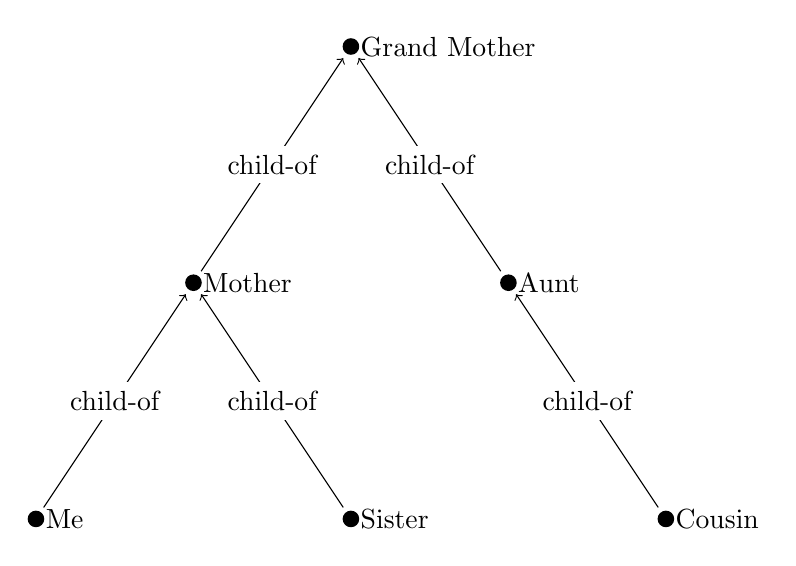
\begin{tikzpicture}
    \coordinate [label=0:{Grand Mother}] (GM) at (4,6);
    \coordinate [label=0:{Mother}] (M) at (2,3);
    \coordinate [label=0:{Aunt}] (A) at (6,3);
    \coordinate [label=0:{Me}] (X) at (0,0);
    \coordinate [label=0:{Sister}] (S) at (4,0);
    \coordinate [label=0:{Cousin}] (C) at (8,0);

    \fill (GM) circle (3pt);
    \fill (M) circle (3pt);
    \fill (A) circle (3pt);
    \fill (X) circle (3pt);
    \fill (S) circle (3pt);
    \fill (C) circle (3pt);

    \draw[->, shorten <= 5pt, shorten >= 5pt,] (M) -- (GM) node [midway,fill=white] {child-of};
    \draw[->, shorten <= 5pt, shorten >= 5pt,] (A) -- (GM) node [midway,fill=white] {child-of};
    \draw[->, shorten <= 5pt, shorten >= 5pt,] (X) -- (M) node [midway,fill=white] {child-of};
    \draw[->, shorten <= 5pt, shorten >= 5pt,] (S) -- (M) node [midway,fill=white] {child-of};
    \draw[->, shorten <= 5pt, shorten >= 5pt,] (C) -- (A) node [midway,fill=white] {child-of};
    \end{tikzpicture}
\caption{\textbf{Simple family tree}: a basic hierarchical representation.}
\end{figure}
An illustrative example for models as graphs are family trees.
A family tree represents people and their familial connections.   
Each node of a family tree corresponds to a person, and is labeled with their name.
Each vertex is an instance of the relation \textit{is a child of}.

\begin{figure}[!h]
    \centering
    \begin{tikzpicture}[level distance=15mm,
        every node/.style={font=\small},
        level 1/.style={sibling distance=45mm},
        level 2/.style={sibling distance=25mm}]
      \node (S) {S}                              % Sentence
        child {node (NP) {NP}                   % Noun Phrase
          child {node (Det) {Det}
            child {node {this}}}}
        child {node (VP) {VP}                   % Verb Phrase
          child {node (V) {V}
            child {node {is}}}
          child {node (NP2) {NP}
            child {node (Det2) {Det}
              child {node {an}}}
            child {node (N) {N}
              child {node {expression}}}}};
      \end{tikzpicture}      
\caption{Syntatic Tree of \textit{this is an expression}}
\end{figure}
Being able to model expressions and languages is a powerful and fundamental feature of object models.
This graph describes the structure of the expression: \textit{this is an expression}.
Here objects represent syntatic structures, such as N noun, Det determinents, V verb, NP noun phrase, and VP verb phrase.
Here we have two NP, one composde of only a Det, and another composed of a Det followed by a N.

\begin{figure}[!h]
  \centering
  \begin{tikzpicture}[level distance=15mm,
      every node/.style={font=\small},
      level 1/.style={sibling distance=35mm},
      level 2/.style={sibling distance=25mm}]
    \node (E) {=}                              % Root: equals expression
      child {node (ADD) {+}                   % Addition subtree
        child {node (NUM1) {2}}
        child {node (NUM2) {2}}}
      child {node (NUM3) {4}};                % Result
  \end{tikzpicture}
\caption{AST of the expression \textit{2 + 2 = 4}}
\end{figure}
Formal languages are commonly manipulated as Abstract Syntax Trees.
In this figure we see the AST for the expression: \textit{2 + 2 = 4}. 
Here the objects correspond to the different symbols of the expression, and the links show how the symbols are organised.





%%%%%%%%%%%%
% Metamodels
%%%%%%%%%%%%
\subsection{Metamodels}
Metamodels are arguably the most important type of model for model driven engineering.
A metamodel is a model that represents a set of models.
A model from that set is said to \textit{conform to} the metamodel.

\begin{figure}[!h]
    \centering
    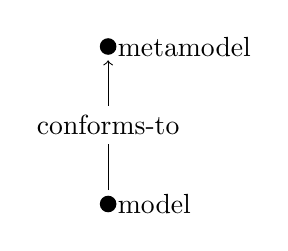
\begin{tikzpicture}
        \coordinate [label=0:{model}] (M) at (0,0);
        \coordinate [label=0:{metamodel}]  (MM) at (0,2);
      
          \fill (M) circle (3pt);
          \fill (MM) circle (3pt);
          
        \draw[->, shorten <= 5pt, shorten >= 5pt,] (M) -- (MM) node [midway,fill=white] {conforms-to};
    \end{tikzpicture}
    \caption{\textit{a model conforms to a metamodel}}
\end{figure}


Metamodels can be formalised with many different languages.
This current section is a simplified metamodel for object and class based modeling, and the following sections are summaries of the UML and OCL metamodels.
For our use-cases, metamodels will come in two parts: 
a collection of class specifications,
and model constraints.
Class specifications define the classes of objects that can be used to make a model 
and define for each class their properties: their attributes and their relations.
Model constraints are use to limit the combinations of objects and the values of their properties.
Model constraints therefore rely on language to query the model.

\subsubsection{Definitions}

\noindent
\textbf{Metamodel}: A metamodel is a tuple $\tuple{M,C}$ where $M$ is a classification model and $C$ is a set of model constraints.

\noindent
\textbf{Conformity}: A model which conforms to a metamodel.

\noindent
\textbf{Classification Model}: Classification models, are a set of classes that maybe be linked to one another.
They are object models representing classification systems: their objects called classes and take a specific form.
% The types of objects in a model conforming to a metamodel are specified in the classification model.
% The types of objects and links are specified in the classification model.

\noindent
\textbf{Class}: Classes represent sets of object, naming them and listing their properties.
For instance, a class can represent and name the concept of a \textit{person}, objects representing people are part of the set the class represents.
The list of properties describe the form objects can take in conforming models.
Classes come in the form of named list of property specifications.
% $$\inlineumlclass{CLASS\_NAME}{\dots}$$

\noindent
\textbf{Property}: a name, type, and collection cardinality.
They specify the information that can be associated with objects.
% $$\inlineumlprop{PROPERTY\_NAME}{TYPE}{m}{n}$$

\noindent
\textbf{Attribute}: named collection of integers associated to an object.

\noindent
\textbf{Reference}: named collection of objects of the model linked to an object.

\noindent
\textbf{Model Constraint}: a constraint expression identifying objects and stating invariants about their combinations or the combination of their properties.
Model constraints are expressions which predicate on the structure of models conforming to the metamodel.
These expressions rely on the vocabulary introduced by the classes and their properties.
Model constraint languages may also provide syntax to navigate a model  

\noindent
\textbf{Meta-Metamodel}:
Metamodels can also be an element of the set they represent, meaning they conform to themselves.
Metamodels can conform to meta-metamodels.

Using the intuition of metamodels as languages: Using the English language, we can describe the English language.

\noindent
\textbf{Domain Specific Language}: 
Domain specific languages are a practical and powerful application of metamodeling.
A powerful intuition for metamodels is that of \textit{metamodels are languages}.
This sentence is an expression which conforms to the vocabulary and the grammar of the English language.
English can be described as a set of words (or bits of words), and rules to combine them.
Expressions in English can represent parts of the real world or abstract ideas.
Domain specific languages leverage this equivalence between metamodels and languages, and use metamodeling frameworks to assist in their development. 
In contrast to general purpose languages (GPL), such as C++, python and Java, DSLs are less expressive but simpler for their given domain.


\subsubsection{Simple Examples of inline notation}
Through out the thesis we'll use inline notation for simple models.
As described above, classes often take the form of named lists of properties.
Taking inspiration from C-like languages, we first name the class, then list the properties between brackets: 
$$\inlineumlclass{CLASS\_NAME}{\dots}$$
Properties are named collections of at least m and at most n elements, of which the elements are typed:
$$\inlineumlprop{PROPERTY\_NAME}{TYPE}{m}{n}$$
Type in our notation is similarly taken from UML standard: \inlineocl(:Type).
Cardinality is noted using intervals: \inlineocl{[m,n]}, where m is minimum cardinality, and n maximum cardinality.

$$\inlineumlclass{Object}{\inlineumlprop{att}{Int}{m}{n}, \inlineumlprop{ref}{Object}{m'}{n'}}$$
This simple metamodel show the general shape of metamodels.
Here we have one class named \inlineocl{Object} representing \textit{objects}.
This class lists two properties: \inlineocl{att} an attribute, and \inelineocl{ref} a reference to other objects in the \inlineocl{Object} class.
Properties being collections, this metamodel also specifies their minimum \inlineocl{m} and maximum \inlineocl{n} number of elements.

$$\inlineumlclass{Person}{\inlineumlprop{age}{Int}{1}{1}, \inlineumlprop{children}{Person}{0}{*}}$$
$$\forall p,q \in \texttt{Person}, p \in q\texttt{.children} \implies p\texttt{.age} < q\texttt{.age}$$
This simple metamodel desribes the person object we've used in previous examples.

% $$\inlineumlclass{Expression}{\inlineumlprop{value}{Int}{1}{1}, \inlineumlprop{subexp}{Expression}{0}{*}}$$
% $$\inlineumlclass{Addition extends Expression}{}$$
% $$\inlineumlclass{Variable extends Expression}{}$$
% $$\forall a\in \texttt{Addition}, |aq\texttt{.subexp}|=2 \wedge a\texttt{.value}= a.q\texttt{.subexp}$$
% This simple metamodel for summation expressions such as $3+4+2$.

%%%%%%%%%%%%
% Model Transformation
%%%%%%%%%%%%
\subsection{Model Validation and Transformation}

% \subsubsection{Model Validation}
\noindent
\textbf{Model Validation}: the process of checking a model conforms to a metamodel.
Models can have errors, because of this modeling tools generally provide a means to leverage the metamodel to check for them.


% \subsubsection{Model Transformation}
\noindent
\textbf{Model Transformation}: 
Model Transformation is the core operation on models.
Model Transformation refers to both the process of transforming models to conform to a new metamodel, and the model of the process.
Model Transformation Execution, generates a target model from a source model according to the MTspec.
Model Transformation Specifications, link classes and properties across metamodels, written in a Model Transformation Language.
Model Transformation Language, generally a super-set of a model constraint language, using query expressions to connect properties and classes.

\begin{figure}[h]
    \centering
    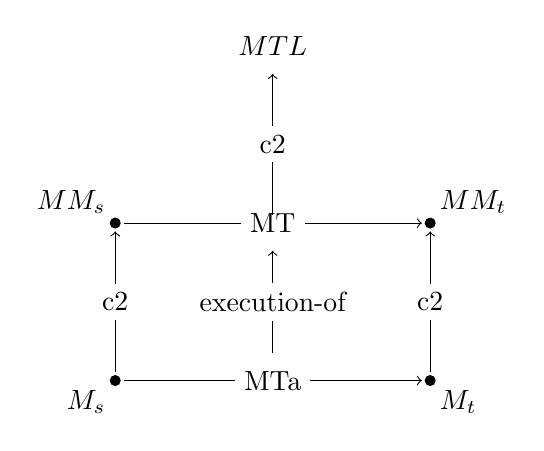
\begin{tikzpicture}
        \coordinate [label=-100:{$M_s$}]  (SM) at (0,0);
        \coordinate [label=-80:{$M_t$}] (TM) at (4,0);
        \coordinate (M2M) at (2,0);
        
        \coordinate [label=100:{$MM_s$}]  (SMM) at (0,2);
        \coordinate [label=80:{$MM_t$}]  (TMM) at (4,2);
        \coordinate (MM2MM) at (2,2);

        \coordinate [label=90:{$MTL$}] (TLMM) at (2,4);
        
            \fill (SM) circle (2pt);
            \fill (TM) circle (2pt);
            \fill (SMM) circle (2pt);
            \fill (TMM) circle (2pt);
        
        \draw[->, shorten <= 3pt, shorten >= 3pt] (SM) -- (TM) node [midway,fill=white] {MTa};
        \draw[->, shorten <= 3pt, shorten >= 3pt] (SMM) -- (TMM) node [midway,fill=white] {MT};
        \draw[->, shorten <= 3pt, shorten >= 3pt,] (SM) -- (SMM) node [midway,fill=white] {c2};
        \draw[->, shorten <= 3pt, shorten >= 3pt] (TM) -- (TMM)node [midway,fill=white] {c2};
        \draw[->, shorten <= 3pt, shorten >= 3pt] (MM2MM) -- (TLMM)node [midway,fill=white] {c2};

        \draw[->, shorten <= 10pt, shorten >= 10pt,] (M2M) -- (MM2MM) node [midway,fill=white] {execution-of};
    \end{tikzpicture}
    \caption{Transformation Pattern}
\end{figure}

A notable group of model transformations includes those which generate code in a programming language.
From a UML Class Diagram, one can generate a Java Class Specification.

\section{The Unified Modeling Language}
% \section{The Unified Modeling Language and the Eclipse Modeling Framework} 
UML provides a range of languages for modeling purposes.
We need languages to describe metamodels and models.
For models, UML provides Object Diagrams, and for metamodels, Class Diagrams and the Object Constraint Language.
Additionally, we will use C-like syntax for Class specifications.

\subsection{Meta-Object Facility}
The Unified Modeling languguage is build ontop of the Meta-Object Facility standard.
Formally: the UML metamodel conforms to MOF meta-metamodel.
MOF provides a meta-metamodel similar to that presented in the previous section.

The MOF standard also describes a four layer model hirearchy illustraiting its application.
The MOF meta-metamodel exists as the top layer of abstraction in the MOF architecture, the M3 layer.
The MOF architecture has three lower layers of abstraction, the lowest being that of the system under study, the M0 layer.
UML exists at the M2 layer, and the M1 layer contains the UML conforming models and metamodels created by the user to represent the system under study.

\begin{figure}[h]
    \centering
    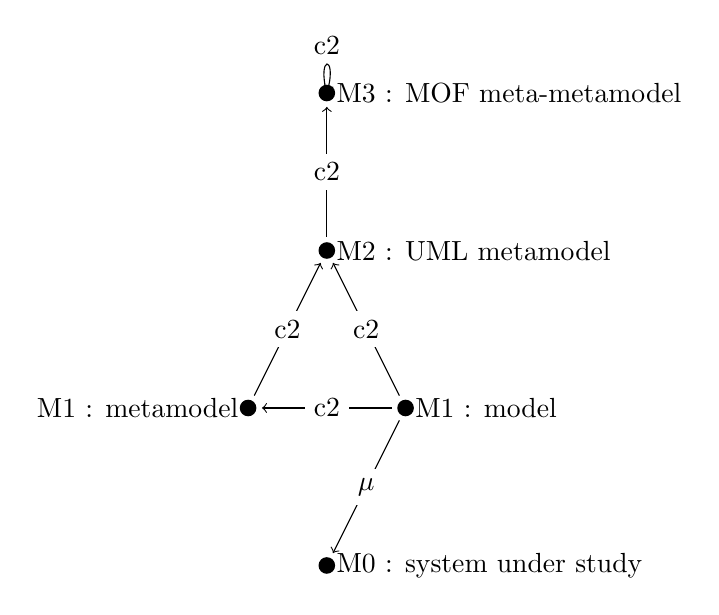
\begin{tikzpicture}
        \coordinate [label=0:{M0 : system under study}] (M0) at (0,0);
        \coordinate [label=180:{M1 : metamodel}]  (M1) at (-1,2);
        \coordinate [label=0:{M1 : model}]  (M12) at (1,2);
        \coordinate [label=0:{M2 : UML metamodel}]  (M2) at (0,4);
        \coordinate [label=0:{M3 : MOF meta-metamodel}]  (M3) at (0,6);

        % \coordinate [label=0:{XMI : model}]  (E1) at (6,2);
        % \coordinate [label=0:{Ecore : metamodel}]  (E2) at (6,4);
        % \coordinate [label=0:{Ecore : meta-metamodel}]  (E3) at (6,6);
      
          \fill (M0) circle (3pt);
          \fill (M1) circle (3pt);
          \fill (M12) circle (3pt);
          \fill (M2) circle (3pt);
          \fill (M3) circle (3pt);

        %   \fill (E1) circle (3pt);
        %   \fill (E2) circle (3pt);
        %   \fill (E3) circle (3pt);
          
        \draw[->, shorten <= 5pt, shorten >= 5pt,] (M12) -- (M0) node [midway,fill=white] {$\mu$};
        \draw[->, shorten <= 5pt, shorten >= 5pt,] (M12) -- (M2) node [midway,fill=white] {c2};
        \draw[->, shorten <= 5pt, shorten >= 5pt,] (M12) -- (M1) node [midway,fill=white] {c2};
        \draw[->, shorten <= 5pt, shorten >= 5pt,] (M1) -- (M2) node [midway,fill=white] {c2};
        \draw[->, shorten <= 5pt, shorten >= 5pt,] (M2) -- (M3) node [midway,fill=white] {c2};

        % \draw[->, shorten <= 5pt, shorten >= 5pt,] (E1) -- (E2) node [midway,fill=white] {conforms-to};
        % \draw[->, shorten <= 5pt, shorten >= 5pt,] (E2) -- (E3) node [midway,fill=white] {conforms-to};
        % \draw[->, shorten <= 5pt, shorten >= 5pt,] (M3) -- (M3) node [midway,fill=white] {conforms-to};
        % \draw (1pt,\y cm) -- (-1pt,\y cm) node[anchor=east] {$\mathbf{\y}$};
        \path[->] (M3) edge [loop above] node {c2} ();
    \end{tikzpicture}
    \caption{Meta-Object Facility model hierarchy}
\end{figure}

\subsection{Class Diagrams}
Class Diagrams identify concepts and their properties.
In a family tree for instance, the core concept is Person, with attributes such as age and references such as parent (or its opposite, child) to express relationships between people. 
%a relation of the person such as \emph{parent} or it's opposite \emph{child} would be a reference type property, an example attribute would be age.

\begin{figure}[!ht]
    \centering
    \includegraphics[trim={0 0 0 0},width=1\linewidth]{Articles/ICTAI2025/figures/metamodel.pdf}
    \caption{UML Class Diagram as Metamodel}
    \label{fig:metamodel}
\end{figure}
In this figure we see a rectangle with a title, which represents a class.
In the rectangle beneath the title, we find a list of attribute properties.
From the rectangle to itself, we see an arrow representing the reference property.
Here we present a generic metamodel.
It describes a class named \inlineocl{Object}, which has two properties: 
\inlineocl{attribute}: a collection of integers, with at least one and at most $m$ elements, \inlineocl{reference}: a collection of up to $n$ references to other \inlineocl{Object} instances.
%\inlineocl{reference} a collection of up to $n$ objects and \inlineocl{attribute} a collection of at least one and at most $m$ integers.
These illustrate the two main types of properties in object-oriented modeling:
Attributes, which store intrinsic data values (e.g., numbers or strings),
References, which define relationships between objects in the model.

%These are illustrative of the two types of object property : references and attributes.
%References describe the relations across a graph of objects, whereas attributes colour the graph nodes.
\subsubsection{UML Collection Types}
UML allows properties to be collections, and distinguishes four standard collection types, based on two dimensions: order and uniqueness.
%Properties are generally collections of elements, and UML distinguishes between 4 concrete collection types: \inlineocl{Sequence}, \inlineocl{Bag}, \inlineocl{OrderedSet} and \inlineocl{Set}.
%hese collection types exist at the intersection between two qualities: orderedness and uniqueness.
\begin{itemize}
    \item \inlineocl{Sequence}: ordered, allows duplicates -- e,g., [2,3,1,1],
   % has ordered non-unique elements:\\ ~[2,3,1,1] has information about order such as \emph{3 before 1}, and repeated values.
    \item \inlineocl{Bag}: unordered, allows duplicates -- e.g., [1,1,2,3], 
    %has non-unique non-ordered elements:\\~[1,1,2,3] has repeated values but we've lost the order.
    \item \inlineocl{Set}: unordered, unique elements only -- e.g., [1,2,3], 
    %has unique non-ordered elements:\\~[1,2,3] has no order and no repeated values.
    \item \inlineocl{OrderedSet}:  ordered, unique elements -- e.g., [2,3,1]. 
    %has order across unique elements:\\ ~[2,3,1] has order but no repeating values.
\end{itemize}
\textcolor{black}{An important note is that \emph{ordered} doesn't pertain to the values.
In [2,3,1,1]: 2 is the \emph{first} value, and 1 is the \emph{last} value. 
}
The intended collection type can be indicated in the class diagram using annotations such as \inlineocl{ordered}, \inlineocl{unique}, or \inlineocl{seq} (for sequences).
%To indicate the collection type of a property in the class diagram, the properties can be annotated with the words \inlineocl{ordered}, \inlineocl{unordered}, \inlineocl{unique}, \inlineocl{ordered} or \inlineocl{seq} (for sequences).
% In modeling tools like the Eclipse Modeling Framework (EMF), class diagrams can be used to automatically generate code. For example, the diagram in Figure \ref{fig:metamodel} could yield the following class definition in an object-oriented programming language:
% %Within a framework such as the Eclipse Modeling Framework, these kinds of diagram can be used to generate code. For instance, from Figure \ref{fig:metamodel} we could generate a class description in an object-oriented programming language:
% \begin{lstlisting}
% class Object {  attribute : int[1..3]
%                 reference : Object[0..2]}
% \end{lstlisting}
% Code generation includes not only class definitions but also methods (getters/setters) and factory mechanisms for instantiating objects and populating models from data sources (e.g., EMF's XMI serialization).
%and generate getters, setters and factories to build these objects when loading data from an EMF model.

% \subsection{Object Diagrams}
% \smallskip
% \noindent \label{ssec:ctxt_id}
\subsubsection{UML Reference Types}
UML also gives us different kinds of relations between objects, notably containment relations and and opposite relations.

\noindent \textbf{Opposite} 
The opposite of \textit{child-of} for instance, is \textit{parent-of}.
Sometimes references may need to be one-way for encapsulation.

\noindent \textbf{Containment} means that the \textit{contained} object is only related to one \textit{container} object through this instance of the relation.



\subsection{Object Diagrams}
% Object diagrams 
describe instances of the classes defined in a class diagram.
%Object (or instance) diagrams show the data, as instances of the concepts described in a class diagram.
For example, Figure~\ref{fig:model} shows an instance conforming to the class diagram in Figure~\ref{fig:metamodel}. It includes three objects, each identified by a unique ID (e.g., \inlineocl{o1}, \inlineocl{o2}, \inlineocl{o3}). For instance, object \inlineocl{o1} has as attribute a collection of 3 integers and is connected to other objects (e.g., \inlineocl{o2} and \inlineocl{o3}).
% Similarly to class diagrams, EMF also supports the use of object diagrams to visually manipulate data instances. 

% which are the maximums allowed by our choice of $n=2$ and $m=3$.

% A family tree is an example of an instance diagram;
% previously, we declared what concepts make up a family tree, but an actual family tree needs instances of related people.
\begin{figure}[!ht]
    \centering
    \includegraphics[trim={0 0 0 0},width=1\linewidth]{Articles/ICTAI2025/figures/model.pdf}
    \caption{UML Instance Diagram as Model}
    \label{fig:model}
\end{figure}
This diagram is also built from rectangles and lines connecting them.
Here each rectangle represents an object, and the title area is used to give the \texttt{:Type} and optionally a name.
Below the title area, we again use the rectangle to list the attributes and the information associated.
The arrows between the rectangles represent instances of the references between objects.
In Figure \ref{fig:model} we see a model which conforms to the metamodel from Figure \ref{fig:metamodel}, for which we chose $n=2$ and $m=3$. This here shows objects of the type described by the class, and the values assigned to their properties.
% This instance will serve to illustrate the result of queries and the operations upon them.
In this model, \inlineocl{o2 : Object} is an instance of the \inlineocl{Object} class named \inlineocl{o2}, as attribute it has a collection of integers with a single value: 1000.
The object \inlineocl{o1} has as attribute a collection of 3 integers and is connected to both other objects, which are the maximums allowed by our choice of $n=2$ and $m=3$.

% These instances can be serialized using the XML Metadata Interchange (XMI) format.
%Similarly to class diagrams, EMF allows us to use object diagrams to manipulate instances of data visually.
%Such an instance would be serialized in the XML Metadate Interchange format.

\section{The Object Constraint Language}
The Object Constraint Language (OCL) is a declarative language used to specify additional rules and constraints on UML models that 
cannot be expressed using diagrams alone. 
It enables the formalization of conditions that instances of the model must satisfy, serving as a powerful complement to class and object diagrams.

Given an instance such as the one shown in Figure \ref{fig:model}, OCL is typically used to verify whether it satisfies the specified constraints. In this work, however, we aim to use OCL as a means to guide model search, thereby enabling the completion or correction of partial or inconsistent data. To this end, we propose an approach that reformulates OCL specifications as constraint satisfaction problems (CSPs). This paper focuses on how OCL’s collection typing, defined in the Class Diagram, and type casting operations can be modeled using global constraints over bounded domains.


\subsection{OCL by example}
OCL is designed to be easy to read an write.
So for an initial introduction we'll use a simple example, and identify the core parts of the language.
The primary use of OCL is to add additional constraints to a class diagram.
% In this subsection we'll build a simple expression which applies to all people: \textit{everyone is younger than their parents}.
% For this we'll be using the following class model:
% $$\inlineumlclass{Person}{\inlineumlprop{age}{Int}{1}{1}, \inlineumlprop{children}{Person}{0}{*}}$$
% And modeling the constraint:
% $$\forall p,q \in \texttt{Person}, p \in q\texttt{.children} \implies p\texttt{.age} < q\texttt{.age}$$

% \section{The Object Constraint Language}
% The Object Constraint Language 

%%
\begin{figure}[!ht]
  \centering
  \includegraphics[trim={0 0 0 0},width=1\linewidth]{Context/MDE/figures/personMM.png}
  \caption{Simple class diagram describing people}
  % \label{fig:model}
\end{figure}
This class diagram describes people, giving their age, and listing their children.

However, a constraint such as \emph{“a child must be younger than their parents”} cannot be represented directly in a class diagram. However, it can be expressed in OCL as follows:
% The Object Constraint Language is used to express specifications that can't be illustrated with Class Diagrams.
% Using OCL we can add more information about the form of a family tree than the class diagram can express.
% For example \emph{a child is always younger than their parents} cannot be expressed in the class diagram, but using OCL we can write the following constraint: 
% \inlineocl{context Person inv: self.parents.age.forall(a | a > self.age)}.
\begin{lstlisting}
context Person inv: 
  self.children.age.forall(a| a < self.age)
\end{lstlisting}
% The most litteral translation of which being: \emph{given any person, that person's children's ages are all less than that of the given person}.
This constraint states that for every Person instance, all of their children must be younger. 
The \inlineocl{context} keyword specifies the class to which the constraint applies, and \inlineocl{inv} stands for \emph{invariant}, i.e., a condition that must always hold true. This invariant states that for every Person, the age of each parent must be greater than the person’s age. 

\subsubsection{self: identidying objects in the model}
%%
% OCL Supports \emph{navigation expressions} (e.g., \inlineocl{self.parents.age}) and \emph{collection operations} (e.g., \inlineocl{forall}, \inlineocl{exists}, \inlineocl{size}) that apply to attributes and references. 
% Table \ref{tab:queries_tgt} shows how different OCL queries evaluate on a sample object model (cf. Figure \ref{fig:model}). 
The expression \inlineocl{self} refers to the current object of the set identified by the context. 
It identified the main variable of the expression. 
\inlineocl{self.attribute} returns its attribute values, and \inlineocl{self.reference} retrieve related objects. 
Chained queries like \inlineocl{self.reference.attribute} retrieve the attributes of referenced objects.


% \subsubsection{self: how ocl expressions are applied to the objects in object models}
% \begin{lstlisting}
%   context Person inv: 
%     self=self
% \end{lstlisting}
% In this listing we see a minimal OCL expression. 
% This expression identifies the context for the constraint \inlineocl{context Person}.
% Contraints in OCL are called \textit{invariants}, and noted \inlineocl{inv}.
% These constraints are applied to every object within the context.
% The objects appear in the expressions using the keyword \inlineocl{self}.

% \begin{lstlisting}
%   context Person inv: 
%     Person.allInstances().includes(self)
% \end{lstlisting}
% We can also access all the object of a class from within a context of any class using \inlineocl{allInstances()} applied to a class name, such as here \inlineocl{Person}.
% This returns a collection of objects that can be iterated upon.
% Here from the context of a single person, we have access to the whole collection of people from the instance.
% Naturally, the person designated by \inlineocl{self} is included. 

% % This example uses the RMS example: from within the context of this invariant on tasks, we predicate using all the 

% For brevity, we simplify this part of these expressions to just the class name.

\subsubsection{Building OCL expressions by chaining operations}
% Now that we have access to the objects of the model, we can start writing expressions to describe our constraint upon them.
OCL expressions a built using function composition.

$$source.operation(arguments)$$
OCL operations generally are applied OCL expressions identified as \textit{source}, which can be understood as the first argument for the operation.
Operation arguments generally take the form of OCL expressions.

\subsubsection{Navigation: relation to the metamodel}
The primary operation on object models, is accessing their properties, and navigating the graph of objects. 
OCL provides language to navigate the model and retrieve it's information.

\noindent
\textbf{Property Access}
OCL uses a \inlineocl{.property} notation for property access.

For example to access the age and the children of a person, in ocl you would write.
$$\inlineocl{self.age}$$
$$\inlineocl{self.children}$$

\noindent
\textbf{Navigation}

To access the children's age, we need to navigate away from the object designated \inlineocl{self}, to the objects representing their parents, and access their age attribute. 

In the general case, if the source expression results in a collection of objects, we can navigate their references to a new collection of objects and access their properties.
$$\inlineocl{source.prop}$$

% \subsubsection{Queries: getting and infering ints and objects from the model}
% Some of the operations will allow us to manipulate collections of objects, such as filtering them or combining them, or summing their attributes.

% \noindent \textbf{Query Expression:} 
% % \inlineocl{self.ref.select(r | predicate(r)).prop.sum()}
% OCL expression resulting in a collection of integers or objects.
% Can be filtered, or merged with other queries.

% \subsubsection{Constraints:  predication upon queries}
% OCL constraints predicated on information inferred from the model, via property access or query expressions.
% % The satisfaction of constraints can also be part of information inferred from the model, and subsequently used in constraints enforced upon the model.
% % This kind of behavior can be found in an expressions such as \inlineocl{self.x < 3 implies self.x=2}

% % \noindent \textbf{Constraint Expression:} 
% % any expression that resolves to a single boolean.
% % Examples of such expressions are where the top operation of the AST is: forall, <, includes.

% \noindent \textbf{Enforced Constraint:} any boolean expression that must resolve to True, such as invariants.

% \noindent \textbf{Topological Constraint:} 
% % \inlineocl{self.ref.prop > self.prop}
% Otherwise referred to as a Structural Constraint, predicates over the relations between objects with respect to their properties.
% \inlineocl{self.children.age.forall(a| a < self.age)} is a topological, as it 

% This is in contrast 

% The top of this expression defines its type and context: \inlineocl{context Person} means this applies to all objects of the \inlineocl{Person} class, and \inlineocl{inv} stands for \emph{invariant}, meaning a statement which is always true.
% Among the sub-expressions of this constraint we find two queries: \inlineocl{self.age} the age of the given person, and \inlineocl{self.parents.age} the ages of their parents.
% This means of querying the instance is core to the object constraint language.
% \begin{table}[!t]
% \centering
% \begin{tabular}{|l|l|l|l|}
% \hline
% \textbf{expression * context} & \textbf{o1} & \textbf{o2} & \textbf{o3}\\ \hline
% % self            & 1         & 2         & 3         \\ \hline
% % self.attribute  & [-3,4,6]  & [1000]    & [-99,-33] \\ \hline
% self.reference  & [3,   2]     & []        & [1]       \\ \hline
% self.reference.attribute      &[-99,-33,1000]&[]&[-3,4,6]\\ \hline
% \end{tabular}
%     \caption{Results of queries (first column) on the instance from Figure \ref{fig:model}}
%     \label{tab:queries_tgt}
% \end{table}
% \begin{table}
% \centering
% \begin{tabular}{|l|l|l|l|l|}
% \hline
% \textbf{expression * context} & \textbf{o1} & \textbf{o2} & \textbf{o3} & \textbf{o4} \\ \hline
% self            & 1         & 2         & 3         & 4     \\ \hline
% self.attribute  & [-3,4,6]  & [1000]    & [-99,-33] & []    \\ \hline
% self.reference  & [3,2]     & []        & [1]       & []    \\ \hline
% self.reference.attribute      &[-99,-33,1000]&[]&[-3,4,6]&[]\\ \hline
% \end{tabular}
%     \caption{Results of queries on the Instance}
%     \label{tab:queries}
% \end{table}
% In Table \ref{tab:queries_tgt} we can see the results of some queries on the instance in Figure \ref{fig:model}.
% Starting with the query \inlineocl{self}, we get the object for which the expression is being interpreted, or in our case an identifier for the object. 
% The queries \inlineocl{self.attribute} and \inlineocl{self.reference} retrieve the information found in Figure \ref{fig:model} for each object.
% For \inlineocl{self.reference} like \inlineocl{self}, we retrieve the identifier of the referenced objects.
% And finally, we have the query \inlineocl{self.reference.attribute} that retrieves the attributes of the objects resulting from \inlineocl{self.reference}.

\subsection{OCL Operations summary}
OCL supports a rich set of operations on primitive types and collections. Examples include: 
\emph{Boolean expressions} (\inlineocl{forall}, \inlineocl{exists}, \inlineocl{not}, \inlineocl{and}, \inlineocl{or}), 
\emph{Arithmetic and comparison} (\inlineocl{+}, \inlineocl{-}, \inlineocl{>}, \inlineocl{<}), and \emph{Collection operations} (\inlineocl{sum}, \inlineocl{size}, \inlineocl{includes}, \inlineocl{asSet}, \inlineocl{asSequence}, etc). Each collection type comes with its own operations and can be explicitly cast using operations like \inlineocl{asSet()}.

\begin{figure}[!ht]
  \centering
  \includegraphics[trim={0 0 0 0},width=1\linewidth]{Context/MDE/figures/oclcheatsheet.png}
  \caption{snippet from the OCL Cheat Sheet provided by eScribis}
  % \label{fig:model}
\end{figure}
This cheat sheet outlines all the available OCL expressions, organized by the types the can be applied to.
% \ytodo{OCL provides lots of operations}
% OCL also provides operations, such as \inlineocl{forall} and \inlineocl{>} seen in the family tree constraint, but also integer and collection operations such as \inlineocl{sum}, \inlineocl{size}.
% Each collection type also comes with their operations, and there are operations to cast a collection from one type to another.
% \ytodo{put as example env}

% The following example enforces that each cage contains animals of at most one species. This constraint involves casting the collection to a \inlineocl{Set} to eliminate duplicates, followed by a cardinality check on the resulting collection. To achieve this, the model is queried for the species of animals present in a given cage using \inlineocl{self.animals.species}. The result is then cast to a set to eliminate duplicates, and the constraint ensures that this set contains at most one element by checking \inlineocl{.asSet().size()<2}.
% %a constraint on cages in a zoo using both collection type casting and an operation on the resulting collection to express a constraint: 
% \begin{lstlisting}
% context Cage inv:
%   self.animals.species.asSet().size() < 2
% \end{lstlisting}
% The constraint requires that there be only one species of animal per cage.
% To do so, it queries the model for the species found in a given cage: \inlineocl{self.animals.species}, and requires the result of that query, when interpreted as a set (eliminating values appearing multiple times) to have at most one element: \inlineocl{.asSet().size()<2}.


% Given an instance such as Figure \ref{fig:model}, OCL is normally used to verify it conforms to the additional constraints.
% However, we wish to use this language to guide model search, allowing us to complete or fix data.
% The method we propose here is to reformulate OCL operations using global constraints, and interpret instances and the OCL constraints upon them as constraint satisfaction problems.
% This paper will show how we reformulate the collection typing specified in the Class Diagram and the type casting OCL operations, using global constraints on integers with bounded domains.
% \ytodo{Motivation from here: if we want to verify or fix the data}
% \ytodo{Motivation for this paper, we want to do this in the context of OCL types}
% \ytodo{Converting types can also be useful when describing constraints}

% \noindent \textbf{Property Access:} \inlineocl{self.prop} \inlineoclast{NavigationOrAttributeCallExp}
% For the object designated by \inlineocl{self} retrieve the collection of values named \inlineocl{prop}.




% \noindent \textbf{Mini-OCL:} \inlineocl{context O inv : self.prop.\dots} is often shortened to \inelineocl{O.prop\dots}.
% We will encounter many small examples of model constraint, to save space we sometimes remove the conxtext declaration.

\subsection{Typing OCL Expressions}
Typing is the process of assigning a data type to expressions, variables, and operations in a language. 
It ensures that operations are performed on compatible data types, preventing logical errors and enhancing code clarity. 
In the context of Object Constraint Language (OCL), typing plays a critical role in defining constraints and queries over UML models, ensuring that expressions are both syntactically and semantically valid.
OCL is statically typed, meaning types are checked at compile-time rather than runtime.

\begin{figure}[!ht]
  \centering
  \includegraphics[trim={0 0 0 0},width=1\linewidth]{Context/MDE/figures/oclType.png}
  \caption{OCL Types}
  % \label{fig:model}
\end{figure}
This diagram specifies the type system for OCL.

\inlineocl{InvalidType} represents incorrect OCL expressions.
\inlineocl{VoidType} represents \textit{absent} values. Such as when \inlineocl{self.children} points to no one.
\inlineocl{Class} represents the use of class names from the metamodel in the model constraint expressions.
\inlineocl{DataType} represents the data that can be found in the model, inferred from it, and the literals in the ocl expressions.
\inlineocl{PrimitiveType} represents the type of data that can be used, such as: integers, reals, booleans, strings.
\inlineocl{CollectionType} represents collections of data.



To color our previous ocl expression on the Person metamodel:
$$self.children.forall(c | c.age < self.age)$$
% \inlineocl{self} and \inlineocl{c} are \inlineocl{VariableExp}.
\inlineocl{.children} is of type \inlineocl{CollectionType} 
\inlineocl{.age} resolves to an integer which is a \inlineocl{PrimiteType}.
\inlineocl{forall} and \inlineocl{<} resolve to a boolean which is a \inlineocl{PrimitiveType}.

This is also a decent metric for OCL coverage.
In this thesis we will be mainly focusing expressions which resolve to a CollectionType and the Integer and Boolean PrimitiveType.
We will also have some cases of Class type, notable when handling \inlineocl{Person} in the expression \inlineocl{Person.allInstances()}
We will also have to manage InvalidType and VoidType.

There are also limitations with the standard OCL typing system, especially around invalid and void expressions, and efforts such as OCL# propose a typing system based on relational logic. Similar to Alloy.
In relational logic all expressions are resolve to sets.
Invalid and Void types are essentially encoded as the empty set $\empty$.

\ytodo{we leverage the type system to define CSP / type is checked before building csp}

\subsection{OCL Expression Metamodel}
OCL being a domain specific language in the model driven ecosystem, we naturally have a class diagram modeling the language. \ytodo{explain}
The OCL metamodel describes the "kinds of words" which appear in the OCL language, and the patterns in which they appear.

\begin{figure}[!ht]
  \centering
  \includegraphics[trim={0 0 0 0},width=1\linewidth]{Context/MDE/figures/oclExpressionMM.png}
  \caption{OCL Expression Metamodel (simplified)}
  % \label{fig:model}
\end{figure}
The top level concept is that of an OCL expression: \inlineocl{OclExpression}.
As previously stated, all OCL expressions are typed, hence they all inherit from the concept of \inlineocl{TypedElement}.

To color our previous ocl expression on the Person metamodel:
$$self.children.forall(c | c.age < self.age)$$
\inlineocl{self} and \inlineocl{c} are \inlineocl{VariableExp}.
\inlineocl{.children} and \inlineocl{.age} are \inlineocl{FeatureCallExp}.
\inlineocl{forall} is a \inlineocl{LoopExp}.
\inlineocl{<} is a \inlineocl{CallExp}.


The \inelineocl{CallExp} represents most of the words in ocl, notably model navigation and operation calls.
Generally an \inelineocl{CallExp} has a source \inlineocl{OclExpression} to which it is applied.
The simplest operations represented by \inlineocl{CallExp} are those applied to primitives, such as arithmetic operations for integers, and logical operations on booleans and integers: +,<,$\wedge$.
The \inlineocl{FeatureCallExp} represents property access, providing attribute values and the objects resulting from references.
Naturally the type of what is returned from property access varies greatly.

The \inlineocl{LoopExp} groups operations applied to expressions of type \inlineocl{Collection}, notably \inelineocl{iterate}, and its special cases such as: \inelineocl{sum}, \inlineocl{size}, \inelineocl{forall}, etc\dots which make up the majority of the collection operations.
The \inlineocl{LoopExp} generally has a \inlineocl{body:OclExpression}, except for builtins such as \inlineocl{sum}. 
If a \inlineocl{LoopExp} has a body, it requires an \inlineocl{interator:Variable}.



The expressions of type \inlineocl{TypeExp}, resolve to OCL types and Classes defined in the metamodel. Notably used in expressions such as \inlineocl{Person.allInstances()}, or \inlineocl{src.select(e|e.oclisTypeof(Person))}, in which \inlineocl{Person} is a \inlineocl{TypeExp}.

The \inlineocl{LiteralExp} allows users to write literal expressions such as \inlineocl{3} or \inelineocl{Sequence(2,1,3,1)}.
The \inlineocl{IfExp} exists for compatibly with older version and can be replaced by \inlineocl{implies}.

The expressions of type \inlineocl{MessageExp} and \inlineocl{StateExp} are not covered in this thesis.

\subsection{OCL Queries and Constraints}
In this thesis we often categorize OCL expressions as either \textit{queries} or \textit{constraints}.

\noindent \textbf{Query Expression:} 
\inlineocl{self.ref.select(r | predicate(r)).prop.sum()}
OCL expression resulting in a collection of integers or objects.

\noindent \textbf{Constraint Expression:} 
\inlineocl{inv: self.ref.forall(r | p(r))}
OCL expression resulting in a boolean.
Constaint expressions can be \textit{enforced} or \textit{reified}.
In this invariant the \textit{forall expression} \inlineocl{self.ref.forall(...)} is enforced, and the \textit{predicate} \inlineocl{p} can be said to be a reified constraint.

% In this thesis we'll many be focusing on \inlineocl{OperationCallExp} which are of type \inlineocl{CallExp}.
% For this we will have to consider \inlineocl{VariableExp}.


\section{EMF and ATL: State-of-the-Art}
\subsection{Eclipse Modeling Framework}
The Eclipse Modeling Framework is a suite of tools for the Eclipse ecosystem, allowing users design data structures, manipulate structured data and generate code.
% At it's core EMF provides an implementation of Essential MOF (EMOF).
% EMOF is also a description of EMF's implementation of Complete MOF.
% EMF provides a specification for Ecore.

\begin{figure}[!ht]
  \centering
  \includegraphics[trim={0 0 0 0},width=1\linewidth]{Context/MDE/figures/emf.png}
  \caption{Using the Eclipse Modeling Framework to edit an Ecore metamodel using a Class Diagram editing tool}
  \label{fig:modelsearch}
\end{figure}
In this screenshot we can EMF being used to create a Class Diagram to design a zoo application.
From this metamodel, we'll be able to generate a tool to edit object models representing instances, and serialize them in XMI files.


\noindent
\textbf{XMI} XML Metadata Interchange, a file format specified by OMG for the serialization of MOF Models.
EMF provides tools to load and save models from and to XMI files.
% EMF provides tools to visualize and manipulate these models.
Loading an XMI model into and EMF editor generally requires the Ecore metamodel it conforms to, and generates EObjects which can be manipulated.
\begin{listing}[!h]
  \begin{lstlisting}[language=xml]
  <Model>  
      <object att="information one" ref="//@object.1"/>
      <object att="information two" ref="//@object.0"/>
  </Model>
  \end{lstlisting}
  \caption{Minimal Object Model in the XMI format}
\end{listing}
In this listing we see a simple model, with two linked objects, each object holds some information.
% It is specified in an XML-like markup language called XML Metadata Interchange.
% XMI is the standard for serialising MOF models.


\noindent
\textbf{Ecore} is the EMF format for class models (metamodels).
Ecore is an XML-like language based on XMI.
% Ecore allows for Class Specifications.
% Ecore can also include OCL expressions, however they can also be provided in a simple text file.
Loading an Ecore file entails instantiating EObjects of type EClasses, EAttributes and EReferences corresponding to the classes of the class model and their properties, and generating code to manipulate them and their corresponding objects.
EMF provides tools so visualize these metamodels as Class Diagrams.

TODO: Add Ecore metamodel.

\noindent
\textbf{EObject} java interface representing objects.
Provides access to the EClass it conforms to.
Provides access to the information via \textit{getters} and \textit{setters}, and the EReference or EAtrribute representing the class property.

\noindent
\textbf{EClass} java interface representing classes.
EClasses provide access to the properties.

\noindent
\textbf{EReference} java interface representing properties of type reference.
Provides access to the name, type, and collection cardinality.

\noindent
\textbf{EAttribute} java interface representing properties of type attribute.
Provides access to the name, type, and collection cardinality.

% \noindent
% \textbf{Model Validation} One of the core features when building models using EMF.
% EMF can validate conformity between a model (XMI file) and metamodel (Ecore and optionally OCL files). 
% As a user builds a model using EMF tools, they can validate that model against the metamodel.
\subsection{Atlas Transformation Language}
% The Atlas Transformation Language provides a means to specify model-to-model transformations in EMF.
The Atlas Transformation Language (ATL) provides a powerful framework for specifying model-to-model transformations within the Eclipse Modeling Framework (EMF). 
ATL is designed to automate the conversion of models from one metamodel to another, enabling the creation of model transformation pipelines—a critical feature for modern Model-Driven Engineering (MDE) workflows.
% ATL can be  to chain model to model transformations allowing for automated modeling pipelines.
% ATL extends OCL to define rules in the context of multiple Classes.
ATL extends OCL (Object Constraint Language) to define transformation rules that operate across multiple classes. These rules establish bindings, which associate properties between source and target model elements using OCL queries. This allows ATL to express complex mappings between metamodels in a declarative style, focusing on what should be transformed rather than how.
These rules associate properties across the classes using OCL queries, in what is called: a binding.

Just like OCL, ATL can be written declaratively, but ATL also allows for imperative sections, which are sometimes necessary to specify \textit{steps} required to transform an object into another.

% $$\inlineocl{rule A from s:Session to r:Rectangle (r.text <- s.name)}$$
% $$\inlineocl{rule B from w:Week to r:Rectangle (r.contains <- A(w.sessions))}$$
% Here we see two simplified rules which describe a transformation from the Scheduling example to the GUI example.
% Rule A describes how to make a GUI element from a session in the schedule.
% Rule A shows a simple binding \inlineocl{r.text <- s.name} between the text of a rectangle and the name of a session.
% Rule B describes how to make a GUI element from a week in the schedule.
% \inlineocl{w.sessions} is the collection of sessions assigned to a week.
% \inlineocl{A(w.sessions)} is the result of rule A applied to the prior collection, which is a collection of rectangles.
% Finally we bind \inlineocl{r.contains} of the resulting rectangle to the resulting collection.

% \begin{lstlisting}
%     // Book.metamodel
%     class Author {
%         name : string;
%         first_name :string;
%     };
    
%     class Book {
%         title : string;
%         author : Author;
%         year : int;
%     };

%     // BookEntry.metamodel
%     class BookEntry {
%         title : string;
%         authorName: string; // Flattened from Author
%         int publicationYear;
%     };
% \end{lstlisting}
\begin{figure}[!ht]
    \centering
    \begin{subfigure}[t]{0.70\linewidth}
        \centering
        \includegraphics[trim={0 0 0 0},width=1\linewidth]{Context/MDE/figures/personANDbookMM.png}
        \caption{Source metamodel: people and books}
    \end{subfigure}
    \hfill
    \begin{subfigure}[t]{0.26\linewidth}
        \centering
        \includegraphics[trim={0 0 0 0},width=1\linewidth]{Context/MDE/figures/BookEntryMM.png}
        \caption{Target metamodel: library book entry}
    \end{subfigure}
\end{figure}
In these two figures we find a source and a target metamodels.
The source metamodel describes books and their relation to people.
And the target metamodel is a specification for a book entry in a library.


\begin{lstlisting}
    // ATL transformation rule
    rule BookToBookEntry {
    from
        b : BookMM!Book
    to
        be : LibraryMM!BookEntry (
            title <- b.title,
            authorName <- b.author.family_name.toUpperCase() + b.author.name,
            year <- b.year
        )
    }
}
\end{lstlisting}

In this example, we focus on a transformation rule, which produces \inlineocl{BookEntry} objects from \inlineocl{Book} objects and their associated \inlineocl{Person} objects.
A rule has two parts: a \inlineocl{from} section which identifies source classes and \inlineocl{to} which identify target classes, and binds their properties to those of the source.  
In the binding \inlineocl{authorName <- b.author.name + b.author.first\_name}, we link the \inlineocl{authorName} property of an entry \inlineocl{be}, to the conjunction of the \inlineocl{name} and \inlineocl{family\_name} of the \inlineocl{Person} identified by the \inlineocl{author} property of the book \inlineocl{b}.

% \section{Examples of Metamodels used in this Thesis}
% \newpage
\subsection{Generic Example}
\begin{figure}[!ht]
    \centering
    \includegraphics[trim={0 0 0 0},width=1\linewidth]{Articles/ICTAI2025/figures/metamodel.pdf}
    \caption{UML Class Diagram as Metamodel}
\end{figure}
This figure present a generic class specification. It describes a class named \inlineocl{Object}, which has two properties: 
\inlineocl{attribute}: a collection of integers, with at least one and at most $m$ elements, \inlineocl{reference}: a collection of up to $n$ references to other \inlineocl{Object} instances.
%\inlineocl{reference} a collection of up to $n$ objects and \inlineocl{attribute} a collection of at least one and at most $m$ integers.
These illustrate the two main types of properties in object-oriented modeling:
Attributes, which store intrinsic data values (e.g., numbers or strings),
References, which define relationships between objects in the model.

This example presents a generic metamodel and model. We'll sometimes color it using the \inlineocl{Person} example:
$$\inlineumlclass{Person}{\inlineumlprop{age}{Int}{1}{1}, \inlineumlprop{children}{Person}{0}{*}}$$
$$\forall p,q \in \texttt{Person}, p \in q\texttt{.children} \implies p\texttt{.age} < q\texttt{.age}$$

% \newpage
\subsection{Graphical User-Interface Example}
\begin{figure}[!ht]
    \centering
    \includegraphics[trim={0 0 0 0},width=1\linewidth]{Contributions/VAR/figures/vizmm.png}
    \caption{UML Instance Diagram as Model}
    % \label{fig:model}
\end{figure}
Model Constraints:
% $$\inlineocl{Rectagle.contains.forall(r|r.position[0] < Rectangle.position[0])}$$
% $$\inlineocl{Rectagle.contains.forall(r|r.position[0] < Rectangle.position[0])}$$
% $$\inlineocl{Rectagle.contains.forall(r|r.position[0]+r.dimension[0] < Rectangle.position[0]+Rectangle.dimension[0])}$$
% $$\inlineocl{Rectagle.contains.forall(r|r.position[1]+r.dimension[1] < Rectangle.position[1]+Rectangle.dimension[1])}$$
$$\inlineocl{Rectangle.contains.forall(r|}$$
$$\inlineocl{r.position[0] < Rectangle.position[0]}$$
$$\inlineocl{r.position[0] < Rectangle.position[0]}$$
$$\inlineocl{r.position[0]+r.dimension[0] < Rectangle.position[0]+Rectangle.dimension[0]}$$
$$\inlineocl{r.position[1]+r.dimension[1] < Rectangle.position[1]+Rectangle.dimension[1])}$$

This metamodel serves as a simplification of a graphical user interface.
The GUI is made up of rectanglular shapes contained within one another (windows, widgets, buttons, etc..).

The class specification declares Rectangle as the sole type of object, and delares their properties to be integer values: x,y position, hight and width.
Additionally the Rectangle specification add a text attribute, containg the text displayed in the rectangle.
The model constraints predicate on the positions and dimensions of contained rectagles and their containing rectagle.
% \newpage
\subsection{Reconfigurable Manufacturing Example}
\begin{figure}[t]
    \includegraphics[trim={0 0 0 0},scale=0.8]{Articles/SAC2025/figures/uc_uml.pdf}
    \caption{Class Diagram for RMS Task constraints} \label{fig:uc_uml}
    \Description[class diagram of RMS]{}
\end{figure}

This figure uses a class diagram to describe the concepts of an RMS, and how they relate (inspired by~\cite{Wang2012-srms}). In this figure, we focus on the graph structure of the model (classes and references among them), omitting attributes. We use the class diagram flavor from the Eclipse Modeling Framework (EMF)\footnote{\url{https://eclipse.dev/modeling/emf/}}, that connects classes by unidirectional \emph{references}, instead of bidirectional \emph{associations}. 

% \footnote{In the use case we're taking inspiration from, all the machines had the same characteristics. We chose an arbitrary number of characteristics to illustrate possible sizes of the resulting CSPs.}
%From it we take 
%the number of stages and tasks to get information about problem sizes, 
%the task precedence tree,
%and an estimate number of machines.
% Larger than the number of stages, smaller than the number of machines.
% equal to the max cardinality of our problem. 
% \ttodo{last two sentences read weird ?}
% \ttodo{I don't understand last part of this sentence}
% Because of the constant nature of the relations linking tasks, machines and characteristics, the optimal implementation doesn't ask the CP solver to compute those matches. 
% In light of this, for our particular use case,  the number of characteristics doesn't have to effect the final size of the CSP. 
% \ttodo{werll, this could be rewritten in a simpler way}

The two main components of a reconfigurable manufacturing system are stages, and machines which are organised into stages.
% Stages have three properties of which two are attributes (stageId and maxMachines) and one is a containment reference to machines.
% Stages are totally ordered and have a numeric label to materialise it, the stageID.
% Common practice in RMS is to label them 10, 20, and so on.
% Thus we represent it as an attribute.
% Additionally, each stage has a maximum number of machines.
A \texttt{Machine}'s property is its relation to a set of \texttt{Characteristics}.
% and for each machine a cost attribute.
% All the machines of a stage must share the same characteristics.
Objects of type \texttt{Task} are partially ordered, as expressed by the \texttt{prev} reference.
%, this order introduces precedence constraints, not addressed here.
% modeled by the prev reference.
% Which  to our problem.
Tasks have two other properties: a reference to a \texttt{Stage} (allocating the task to that stage), and a reference to characteristics (i.e., the machine characteristics needed to perform the task). Similarly to the example in \cite{Wang2012-srms}, tasks and machines can be linked to any number of characteristics.

\subsubsection {OCL Constraints for RMS}

\begin{listing}
\begin{lstlisting}[language=ocl]
context Task inv SameCharacteristicConstraint: 
    self.stage.machines.forall(m | m.characteristics
        ->includesAll(self.characteristics)) 

context Task inv PrecedenceConstraint: 
    self.stage.stageNum >= self.prev.stage.stageNum
\end{lstlisting}
\caption{RMS Task constraints in OCL.} \label{lst:uc_ocl}
\end{listing}
% \newpage
\subsection{Zoo Example}
\begin{figure}[!ht]
    \centering
    \includegraphics[trim={0 0 0 0},width=1\linewidth]{Articles/ICTAI2025/figures/zooMM.pdf}
    \caption{Zoo Metamodel}
\end{figure}
\begin{lstlisting}
    context Cage inv:
        self.animals.species.asSet().size() < 2
    and self.animals.species.space.sum() <= self.capacity
\end{lstlisting}

In this example we have a simple metamodel for a Zoo.
% \newpage
\subsection{Scheduling Example}
\begin{figure}[!ht]
    \centering
    \includegraphics[trim={0 0 0 0},width=1\linewidth]{Contributions/VAR/figures/schedulingmm.png}
    \caption{UML Instance Diagram as Model}
    % \label{fig:model}
\end{figure}
$$\inlineocl{Session.requisite.forall(r|r.week.number < Session.week.number)}$$
$$\inlineocl{Session.corequisite.forall(r|r.week.number = Session.week.number)}$$

In \ytodo{this figure} we see an example metamodel for a schedule.
We have as concepts sessions and weeks.
Weeks are identified by a week number.
Sessions are assigned to weeks, and have prerequisite sessions that must be done during a prior week, and correcquisite sessions which must be done the same week.